\documentclass[12pt]{article}
\usepackage{sbc-template}
\usepackage{graphicx,url}
\usepackage[export]{adjustbox}
\usepackage[brazil]{babel}
\usepackage[utf8x]{inputenc}
\usepackage{url}  % para usar URLs nas referencias
\sloppy

% Relatos de experiência: artigos de alta qualidade descrevendo e analisando a aplicação de processos, métodos ou ferramentas de qualidade de software, contextualizando a experiência e mostrando os resultados obtidos e lições aprendidas, em uma experiência prática com contribuição para a indústria de software
% max de 8 paginas
%http://www.softex.br/wp-content/uploads/2013/09/Como-escrever-um-relato-de-experi%C3%AAncia.pdf

\title{Automação de Testes em Aplicações de BPMS:\\ um Relato de Experiência}

\author{Jessica Lasch de Moura\inst{1},
Andrea Schwertner Charão\inst{1}}
\address{Núcleo de Ciência da Computação\\
Universidade Federal de Santa Maria -- UFSM
\email{\{jmoura, andrea\}@inf.ufsm.br}}

\begin{document}

\maketitle

\begin{resumo}
Este artigo relata uma experiência de teste automatizado de uma aplicação desenvolvida com o apoio de sistemas de gestão de processos de negócio (Business Process Management Systems -- BPMS). Para isso, implementou-se um mesmo processo em dois diferentes BPMS: Bonita e Activiti. Buscou-se submeter este processo a dois tipos de teste: testes de carga e testes funcionais, utilizando-se as ferramentas de teste Apache JMeter, Cucumber e Selenium. Os resultados evidenciam limitações e oportunidades na automação de testes deste tipo de aplicação.
\end{resumo}
% limitações, oportunidades e ... (o que deu certo e o que não deu)

\begin{abstract}
This article discusses the automated testing of applications developed with the support of Business Process Management Systems -- BPMS. We present an experience report on the automation of load tests and functional tests over a real BPM application, using the Apache JMeter and Selenium open-source tools. Results show the limitations and opportunities in test automation of BPM applications.
\end{abstract}

\section{Introdução}

A gestão de processos de negócio (\emph{Business Process Management} -- BPM) tem suscitado o interesse de empresas e da comunidade científica, tanto por seus benefícios como por seus desafios. Designa-se por BPM o conjunto de conceitos, métodos e técnicas para suportar a modelagem, administração, configuração e análise de processos de negócio~\cite{weske, aalst2013survey}. Associados a isso, surgiram os sistemas BPM (\emph{Business Process Management Systems} ou \emph{Suites} -- BPMS), que são ferramentas de software para apoio ao ciclo de vida da gestão de processos de negócio. Tais ferramentas, quando bem aplicadas, têm o potencial de alavancar aumentos de produtividade e redução de custos nos mais variados tipos de organizações. 

Dentre os diversos BPMS disponíveis atualmente, é comum encontrar ferramentas com suporte a modelagem, configuração e execução de processos de negócio. Por outro lado, tarefas relacionadas à simulação, monitoramento, verificação e testes ainda são consideradas um desafio nesta área~\cite{aalst2013survey}. Em particular, o teste automatizado de aplicações de BPM é pouco abordado, tanto pela comunidade da área de BPM~\cite{aalst2013survey} como da área de testes de software~\cite{graham2012experiences}. Diante disso, estima-se que muitas organizações se limitem a testes manuais em suas aplicações de BPM. No entanto, a falta de automação nos testes pode levar a vários problemas durante a implementação e execução de processos de negócio, como baixa aderência aos requisitos, maior esforço dos desenvolvedores, desperdício de tempo e aumento do risco de duplicação de esforços e de erro humano. 

Nesse contexto, o presente artigo relata uma experiência de automação de testes em uma aplicação de BPM desenvolvida para agilizar um processo em uma instituição pública de ensino. Todas as etapas do desenvolvimento da aplicação, utilizando o BPMS Bonita Open Solution (BOS), foram apresentadas em um trabalho precedente~\cite{sbsi2013}. 

\section{BPM e Testes}

Em muitos casos, o termo BPM pode ser usado com significados diferentes~\cite{acmxrds2009}, às vezes com mais ênfase em tecnologia (software) e outras vezes mais associado a gestão. Mesmo assim, a área tem convergido sobre o ciclo de vida de aplicações de BPM, que envolve as atividades de análise, modelagem, execução, monitoramento e otimização~\cite{ABPMP}. 

%Os sistemas de BPM (BPMS) têm se afirmado como ferramentas essenciais para suporte a atividades desse ciclo de vida. Atualmente, pode-se dizer que um típico BPMS oferece recursos para definição e modelagem gráfica de processos, controle da execução e monitoramento de atividades dos processos. Alguns exemplos de BPMS que se destacam neste cenário são IBM Websphere ~\cite{WEBSPHERE}, Oracle BPM Suite~\cite{ORACLEBPM}, Intalio~\cite{INTALIO}, Bizagi~\cite{BIZAGI}, TIBCO BPM~\cite{TIBCOBPM}, Activiti~\cite{ACTIVITI} e Bonita Open Solution ~\cite{BONITASOFT}.
% Referencias acima foram retiradas por ocuparem muito espaco no final. Podem ser substituidas por notas de rodape, caso haja espaco.

%Os sistemas de BPM (BPMS) têm se afirmado como ferramentas essenciais para suporte a atividades desse ciclo de vida. Atualmente, pode-se dizer que um típico BPMS oferece recursos para definição e modelagem gráfica de processos, controle da execução e monitoramento de atividades dos processos. Alguns exemplos de BPMS que se destacam neste cenário são IBM Websphere, Oracle BPM Suite, Intalio, Bizagi, TIBCO BPM, Activiti e Bonita Open Solution.

Os sistemas de BPM (BPMS) têm se afirmado como ferramentas essenciais para suporte a atividades desse ciclo de vida. Atualmente, pode-se dizer que um típico BPMS oferece recursos para definição e modelagem gráfica de processos, controle da execução e monitoramento de atividades dos processos. Nota-se que a preocupação com testes não fica evidente na ferramentas BPMS. De fato, analisando-se o material promocional e a documentação publicamente disponível sobre os principais BPMS, observa-se uma ênfase em etapas de modelagem e execução.

%Nota-se que a preocupação com testes não fica evidente na ferramentas BPMS. De fato, analisando-se o material promocional e a documentação publicamente disponível sobre os principais BPMS, observa-se uma ênfase em etapas de modelagem e execução. Visivelmente, tais recursos são um diferencial no desenvolvimento de aplicações de BPM, em comparação ao desenvolvimento de software em geral. No entanto, aplicações de BPM também estão sujeitas a defeitos e, por isso, podem se beneficiar de avanços na área de testes de software.

%Em engenharia de software, o teste é tradicionalmente considerado uma prática importante~\cite{pressman, swebok}. Há uma vasta terminologia relacionada a testes de software, classificando-os de acordo com diferentes critérios (objetivos, técnicas, entre outros). Por exemplo, os testes podem abranger o sistema inteiro (teste de sistema), alguns componentes (teste de integração) ou unidades isoladas (teste unitários). Alguns autores também distinguem testes funcionais, que avaliam o comportamento do software frente a seus requisitos, dos testes ditos não-funcionais, que verificam atributos relacionados aos requisitos não-funcionais do software, como por exemplo desempenho e usabilidade~\cite{desikan2006software}. Técnicas de teste podem variar de acordo com a natureza da aplicação~\cite{swebok}, por exemplo: orientada a objetos, baseada na Web, com interface gráfica, etc.
% citar livro do Cem Kaner

Em testes de software, há muitas tarefas que podem ser trabalhosas e propensas a erros quando realizadas manualmente. Por este fato, vários autores relatam a importância dos testes automatizados em ambientes de desenvolvimento~\cite{sbqs2013}. Assumindo que aplicações de BPM podem ser tratadas como software em geral, é possível testá-las sob diferentes aspectos, por meio de tipos de testes já consagrados em engenharia de software, como por exemplo testes funcionais do tipo caixa-preta ou teste de carga. Sob esta ótica, pode-se empregar ferramentas de automação de testes alinhadas com cada tipo de teste. No entanto, a adoção esta abordagem pode ter limitações e dificuldades, pois não leva explicitamente em conta o ciclo de vida de aplicações de BPM.


%Com a evolução das áreas de qualidade e teste de software, foi surgindo uma variedade de soluções para automação de testes. Ferramentas para testes unitários, por exemplo, são numerosas e costumam se integrar aos ambientes de desenvolvimento~\cite{unittesting}. Outro exemplo é o teste de aplicações baseadas em interfaces gráficas ou Web~\cite{webtesting}.

%http://en.wikipedia.org/wiki/List_of_GUI_testing_tools

%Pressman define quatro tipos de teste de software: teste de unidade, teste de integração, teste de validação, teste de sistema. Teste de unidade concentra-se em cada unidade do software, de acordo com o que é implementado no código fonte, utiliza as técnicas de teste de caixa branca e caixa preta. Teste de integração concentra-se no projeto e na construção da arquitetura de software, utilizando principalmente as técnicas de teste de caixa preta. No teste de validação os requisitos estabelecidos como parte da análise de requisitos de software são validados em relação ao software que foi construído. Por último, no teste de sistema, o software e outros elementos do sistema são testados como um todo. Teste de segurança e recuperação \cite{pressman1995engenharia}. O teste de sistema pode ser dividido em uma série de diferentes testes, cujo objetivo principal é por completamente à prova o sistema, dentre estes sub-tipos de testes está o teste de carga.

%Assumindo que aplicações de BPM podem ser tratadas como software em geral, é possível testá-las sob diferentes aspectos, por meio de tipos de testes já consagrados em engenharia de software, como por exemplo testes funcionais do tipo caixa-preta ou teste de carga. Sob esta ótica, pode-se empregar ferramentas de automação de testes alinhadas com cada tipo de teste. No entanto, a adoção esta abordagem pode ter limitações e dificuldades, pois não leva explicitamente em conta o ciclo de vida de aplicações de BPM.

%Há alguns anos, o termo \emph{Business Process Testing -- BPT} vem sendo empregado para designar testes de processos de negócio. Não há uma caracterização clara deste tipo de teste, sendo que em alguns contextos o termo refere-se a testes automatizados reusáveis criados por especialistas do domínio~\cite{hp}, portanto aderentes aos processos de negócio. Em outros contextos, o termo relaciona-se a automação de testes de processos implementados em arquiteturas orientadas a serviços (\emph{Service Oriented Architectures} -- SOA)~\cite{soatest2008, bpeltest2008}. Testes deste tipo possuem uma relação com BPM e são uma especialização de testes de software em geral. No entanto, pode-se dizer que essa relação com BPM é fraca, pois é principalmente focada na etapa de execução dos processos. Além disso, não costumam ser soluções integradas em sistemas BPM.


% sistemas BPMS: simulação, monitoramento...
%http://www8.hp.com/us/en/software-solutions/software.html?compURI=1174789#.UvTvdfjei1H


%Aspectos comuns a qualquer tipo de software
%- verificação (conformidade, corretude, ...)


%Aspectos particulares
%- verificação dos modelos BPMN
%- caminhos críticos e gargalos (simulação)


%Os desafios da homologação de Processos Automatizados
%http://blog.iprocess.com.br/2013/04/os-desafios-da-homologacao-de-processos-automatizados/


\section{Aplicação Alvo de Testes}

A aplicação alvo deste trabalho refere-se a um processo comum em instituições de ensino superior: a apreciação de Atividades Complementares de Graduação (ACGs), ou seja, atividades que formam a parte flexível do currículo de graduandos (participação em palestras, eventos, projetos, etc.). Em um trabalho anterior ~\cite{sbsi2013}, apresentou-se a modelagem e implantação desse processo. Sua representação em BPMN, na Figura \ref{fig:diagrama}, revela um total de 11 tarefas distribuídas em 5 divisões de responsabilidade (Aluno, Tutor, etc.).

No trabalho anterior, implementou-se o processo com a ferramenta Bonita Open Solution\footnote{Bonita Open Solution. Disponível em: www.bonitasoft.com.}, um BPMS de código aberto reconhecido no mundo corporativo~\cite{gartner, forrester}. A aplicação resultante possui vários formulários Web relativos a cada divisão de responsabilidade, sendo o primeiro deles destinado ao preenchimento de dados pelo aluno. De acordo com o tipo de atividade complementar (eventos, projetos, etc.), o fluxo é direcionado para os responsáveis pela avaliação e validação da ACG. Nota-se, na Figura 1, que o processo possui diversos desvios condicionais, o que leva a mais de 15 caminhos possíveis no processo.

\begin{figure}[ht]
\centering
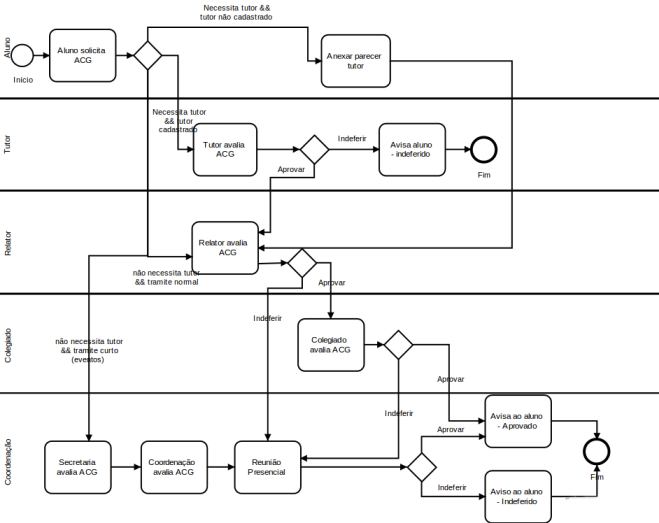
\includegraphics[max size={15cm}{15cm}]{figuras/processo.png}
\caption{Diagrama do processo em BPMN}
\label{fig:diagrama}
\end{figure}

A aplicação foi submetida a testes funcionais realizados manualmente, além de testes de aceitação realizados com um grupo de usuários reais. Entretanto, com algumas semanas em operação, surgiram problemas: instâncias do processo falharam devido a entradas inesperadas, serviços não foram restabelecidos corretamente após serem interrompidos e houve sobrecarga devido ao grande número de casos abertos numa data limite. Essa experiência motivou a busca de soluções para automação de testes.

%, em especial testes de carga e testes funcionais, que supostamente poderiam ter evitado os problemas observados na implantação.

Verificou-se, no entanto, que o BPMS utilizado não possuía suporte a nenhum tipo de teste automatizado. Buscou-se outros BPMS com licenças \emph{open source}, que pudessem implementar o processo em questão e que oferecessem suporte a testes. Dentre as ferramentas analisadas (TIBCO\footnote{TIBCO. Disponível em: www.tibco.com.}, Sydle Seed\footnote{Sydle Seed. Disponível em: www.sydle.com/bpms.}, Activiti\footnote{Activiti. Disponível em: www.activiti.org.}, Process Maker\footnote{Process Maker. Disponível em: www.processmaker.com.}, Intalio\footnote{Intalio. Disponível em: www.intalio.com.}), nenhuma oferecia suporte a testes automatizados, apenas a ferramenta Activiti cita a possibilidade de um teste de unidade aliado ao JUnit porém não existem informações extras sobre essa alternativa. Por isso partiu-se para outra opção: utilizar ferramentas de teste externas ao BPMS. Mesmo assim, decidiu-se implementar a mesma aplicação usando outro BPMS, a fim de ampliar a experiência e, possivelmente, identificar semelhanças e diferenças no teste automatizado de implementações com diferentes BPMS.
A ferramenta escolhida foi Activiti, um BPMS de código-aberto que trabalha com a mesma versão da notação BPMN usada no BOS, permitindo importar na íntegra o processo originalmente criado com o Bonita Open Solution. Os formulários Web, no entanto, não puderam ser importados e foram recriados manualmente.
%, preservando-se as mesmas características.


% capaz de apoiar desde a modelagem até a implantação do processo.

%a ferramenta Bonita Open Solution. Como mostra a Figura \ref{fig:diagrama}. É um processo complexo que permite analisar diversas funcionalidades dos BPMS e, justamente por já ter sido alvo de um trabalho, é um processo no qual já se tem uma grande experiência.



%Devido ao tempo limitado para a conclusão deste trabalho, decidiu-se por escolher duas ferramentas para o estudo. Primeiramente, foi escolhida a ferramenta Bonita Open Solution, devido a esta já ter sido usada em um trabalho anterior ~\cite{sbsi2013} e, por isso, tem se uma vasta experiência nesta ferramenta. O Bonita Open Solution (BOS) é uma ferramenta distribuída sob uma licença de software livre, desenvolvida em Java, pela empresa BonitaSoft~\cite{BONITASOFT}.% A ferramenta BOS oferece componentes tanto para a modelagem como para a implementação e transformação de processos. A modelagem e customização de processos é realizada através do Bonita Studio, um componente com interface gráfica tipo desktop que agrupa ferramentas de desenvolvimento. Também é possível agregar funcionalidades aos processos através de conectores que podem, inclusive, receber personalizações feitas através de códigos.

%Analisando as ferramentas disponíveis e levando em conta os trabalhos e livros publicados ~\cite{rademakers2012activiti} que abordam o uso da ferramenta, o segundo software escolhido foi o Activiti. O Activiti ~\cite{ACTIVITI} é um BPMS de código aberto, distribuído sob uma licença Apache, criado em Java e usa  BPMN 2.0 para a modelagem dos processos, ele pode ser executado em qualquer plataforma, servidor, cluster ou na nuvem. %A ferramenta Activiti oferece componentes distintos para modelagem, implementação e execução de processos. A modelagem e customização dos processos é feita no Activiti Designer que é um plugin para a plataforma Eclipse, o que torna o ambiente de criação fácil de ser usado, a execução é feita no componente chamado Activiti Explorer.

%Na Tabela \ref{tab:tabelaCaminhos} são exibidos todos os possíveis caminhos pelos quais o processo alvo dos testes poderia passar, sendo 'x' a representação de que o caminho passou pela determinada etapa do processo. Esta tabela foi criada durante a implantação da aplicação citada neste trabalho para auxiliar na execução dos testes (que foram executados manualmente quando a aplicação foi implantada).


%\begin{table}
%{\scriptsize
%\begin{tabular}{|p{1cm}|p{1cm}|p{1cm}|p{1cm}|p{1cm}|p{1cm}|p{1cm}|p{1cm}|p{1cm}|p{1cm}|p{1cm}|p{1cm}|}
%\hline
%Aluno Solicita ACG & Anexar parecer tutor & Tutor avalia & Avisa aluno (indeferido) & Rela\-tor avalia & Cole\-giado avalia & Atu\-aliza BD & Secre\-taria avalia & Coorde\-nador avalia & Reuni\-ão presencial & Avisa aluno (indeferido) & Avisa aluno (aprovado) \\\hline
%x & x & - & - & x & x & x & - & - & - & - & x\\\hline
%x & x & - & - & x & x & - & - & - & x & x & -\\\hline
%x & x & - & - & x & x & - & - & - & x & - & x\\\hline
%x & x & - & - & x & - & - & - & - & x & - & x\\\hline
%x & x & - & - & x & - & - & - & - & x & x & -\\\hline
%x & - & x & x & - & - & - & - & - & - & - & -\\\hline
%x & - & x & - & x & x & x & - & - & - & - & x\\\hline
%x & - & x & - & x & x & - & - & - & x & x & -\\\hline
%x & - & x & - & x & x & - & - & - & x & - & x\\\hline
%x & - & x & - & x & - & - & - & - & x & - & x\\\hline
%x & - & x & - & x & - & - & - & - & x & x & -\\\hline
%x & - & - & - & x & x & x & - & - & - & - & x\\\hline
%x & - & - & - & x & x & - & - & - & x & x & -\\\hline
%x & - & - & - & x & x & - & - & - & x & - & x\\\hline
%x & - & - & - & x & - & - & - & - & x & - & x\\\hline
%x & - & - & - & x & - & - & - & - & x & x & -\\\hline
%x & - & - & - & - & - & - & x & - & - & - & x\\\hline
%x & - & - & - & - & - & - & x & x & - & - & x\\\hline
%x & - & - & - & - & - & - & x & x & x & - & x\\\hline
%x & - & - & - & - & - & - & x & x & x & x & -\\\hline
%\end{tabular}
%}
%\caption{Caminhos possíveis}
%\label{tab:tabelaCaminhos}
%\end{table}


\section{Descrição e Execução dos Testes}
No planejamento de testes automatizados, priorizou-se o teste de etapas que de fato revelaram problemas durante a operação.
%Com isso, buscou-se verificar se os problemas poderiam ser facilmente identificados antes de colocar-se a aplicação em produção. 
Os testes escolhidos foram: (a) testes de carga, que são um tipo de teste de desempenho, visando avaliar o comportamento do sistema frente a um grande número de solicitações e (b) testes funcionais, a fim de verificar as saídas do sistema produzidas a partir de entradas pré-definidas. \textbf{Nenhum destes tipos de teste possui suporte nos BPMS Bonita e Activiti}, que incluem somente funcionalidades limitadas de simulação e depuração de execução dos processos. Assim, realizou-se um levantamento de ferramentas externas aos BPMS, destinadas ao teste de aplicações Web. Selecionou-se as julgadas mais promissoras, antes de partir-se para o detalhamento e execução dos testes.

\subsection{Teste de Carga}

Testes de carga em aplicações Web são tipicamente realizados gerando-se múltiplas requisições HTTP ao servidor, de forma controlada. Para isso, uma etapa crítica é a identificação das requisições que devem ser geradas. Existem diversas ferramentas que se propõem a facilitar este tipo de teste, dentre as quais pode-se citar: JMeter\footnote{Apache JMeter. Disponível em: www.jmeter.apache.org.}, The Grinder\footnote{The Grinder. Disponível em: www.grinder.sourceforge.net/.} e WebLOAD\footnote{WebLOAD. Disponível em: radview.com/webload-download/.}. Todas são ferramentas \emph{open source} e possuem diversas opções, mas escolheu-se a ferramenta JMeter pela sua funcionalidade de captura de requisições, por meio da opção "proxy server"".

%a maior desvantagem dessas ferramentas é que não existe a possibilidade de capturar as requisições que devemos testar de uma forma automática, todas requisições precisam ser inseridas manualmente no plano de teste. No JMeter existe a opção 'Servidor de Proxy' que permite capturar o tráfico de requisições e este é automaticamente transformado em requisições no plano de teste.
%Para executar os testes de carga foi selecionada a ferramenta JMeter ~\cite{JMETER}, e escolha desta ferramenta para testar aplicações BPM deu-se por diversos motivos.



Um teste da aplicação com JMeter consiste em quatro etapas: capturar as requisições HTTP, exportar requisições (formato .jrxml para JMeter), configurar o plano de teste e, por fim, executar o teste no JMeter. Dependendo do BPMS utilizado, a aplicação gera diferentes requisições HTTP que precisam ser identificadas e interpretadas, para serem reproduzidas automaticamente. O emprego de tecnologias Web com processamento assíncrono, do lado do cliente, pode dificultar esta etapa, pois uma ação do usuário pode não gerar imediatamente uma requisição ao servidor. Além disso, em aplicações de BPMS, diversos usuários atuam sobre diferentes etapas de um mesmo processo, de modo que as requisições HTTP carregam chaves identificando usuários e processos.

%Ocorrem dois principais problemas na execução do teste de carga em ambas as ferramentas: (a) Captura e interpretação das requisições que utilizam a tecnologia GWT e (b) dependência entre as tarefas do processo, cuja implementação muda conforme o BPMS. 

No caso da aplicação criada com Bonita, verificou-se que existe uma chave identificadora de sessão que é gerada no momento em que usuário acessa o sistema e outra chave identificadora de instância, ou seja, que identifica cada execução do processo como única, sendo criada pelo servidor no momento em que o usuário inicia o processo. Para executar os testes, portanto, foi necessário localizar a requisição em que essas chaves são geradas e utilizar a ferramenta "Extrator de Expressão Regular" do JMeter para obter seus valores. Já na aplicação criada com Activiti, foi inviável identificar a requisição em que as chaves são geradas, pois não há uma requisição cujo retorno (resposta do servidor) contenha valores de chaves. Esta situação leva a crer que a geração das chaves identificadoras é feita internamente pelo BPMS, ou seja, não em uma requisição HTTP e, por consequência, esta não pode ser capturada e reproduzida no JMeter.

\begin{table}
{\scriptsize
\begin{tabular}{|p{5cm}|p{4cm}|p{4cm}|}
\hline
 & BOS & Activiti \\\hline
Captura das requisições usando apenas JMeter & Problemas com GWT & Problemas com GWT\\\hline
Foi possível capturar e exportar as requisições HTTP? & Sim (Utilizando BlazeMeter) & Sim (Utilizando BlazeMeter)\\\hline
Ocorreu problema com dependência das tarefas do processo? & Sim & Sim \\\hline
Foi possível identificar a solução para a dependência das tarefas? & Sim & Não\\\hline
Foi possível configurar e executar os testes? & Sim & Não\\\hline
\end{tabular}
}
\caption{Teste de carga}
\label{tab:testeCarga}
\end{table}



%No caso do teste de carga, foi encontrado um problema para capturar e interpretar requisições que utilizavam a tecnologia GWT (Google Web Toolkit), este problema foi a causa do teste de diferentes ferramentas de captura de requisições e, nesse caso, obteve-se sucesso por meio do uso combinado do servidor proxy do JMeter, com seu recurso de visualização do cabeçalho das requisições e com o BlazeMeter Chrome Extension para capturar as requisições. Outros softwares utilizados para capturar as requisições não suportavam o tratamento a requisições que utilizavam GWT e/ou não permitiam exportar as requisições capturadas diretamente para o formato aceito pelo JMeter (precisavam se inseridas manualmente).

%Outro problema, também exibido na Tabela \ref{tab:bpms2}, ocorreu devido a uma particularidade de sistemas BPM, em que várias tarefas de um processo são dependentes entre si e a forma como isso é implementado muda conforme o sistema. No BOS existe uma chave identificadora de sessão que é gerada no momento em que usuário acessa o sistema e outra chave identificadora de instância, ou seja, identifica cada execução do processo como única, e é criada no momento em que o usuário inicia o processo. Para executar o teste com sucesso, foi necessário localizar a requisição em que essas chaves são geradas, utilizar a ferramenta "Extrator de Expressão Regular" do JMeter para obter o valor da chave, guardar o valor obtido em uma variável do JMeter e então substituir os valores por esta variável em todas as requisições que utilizam as chaves, esta etapa exigiu um estudo mais aprofundado da implementação do processo no BOS e também foi trabalhosa.

%No caso da ferramenta Activiti, as chaves identificadoras também foram encontradas, no entanto, foi impossível identificar em que requisição as mesmas eram geradas, de fato na primeira requisição capturada as chaves já são utilizadas/enviadas ao servidor no contéudo da requisição, ou seja, não havia uma requisição cujo o retorno (resposta do servidor) contivesse as chaves utilizadas. Esta situação leva a crer que a geração das chaves identificadoras é feita internamente pelo BPMS, ou seja, não em uma requisição HTTP e, por sequência, esta não pode ser capturada e importada no Jmeter.


%pode testar com o bonita e com o activiti não
%resultados
\subsubsection{Resultados}
Com o objetivo de obter o comportamento do sistema em diferentes níveis de carga, foram executados testes com 1, 50, 100 e 200 usuários virtuais e foram analisadas as requisições referentes aos seguintes passos: efetuar login, exibir a página inicial do BOS, selecionar o processo, exibir o formulário inicial e enviar o formulário preenchido. Os testes foram executados em um servidor com 24 GB de RAM e 2 processadores Intel Xeon E5520, com 4 núcleos. Foi possível executar o teste de carga apenas na ferramenta Bonita Open Solution, pois o software Activiti demonstrou os problemas relatados acima.

%Reproduzindo o teste com um usuário virtual, nas requisições correspondentes a login, exibição da página inicial, seleção do processo, exibição do formulário inicial e envio do formulário preenchido, a média do tempo de resposta foi de, respectivamente, 126, 32, 38, 80 e 73 milissegundos. A média do tempo de resposta total foi de 75 milissegundos e o desvio padrão foi igual a 21.  Aumentando o número de usuários virtuais para cinquenta os valores do tempo de resposta subiram para 597, 191, 179, 368 e 152 milissegundos, a média foi igual a 329 milissegundos e o desvio padrão 401. Com 100 usuários o aumento do tempo de resposta fica ainda mais visível, sendo 1972, 571, 552, 760 e 694 milissegundos, com média 774 milissegundos e desvio padrão de 1449.


\begin{table}
{\scriptsize
\centering
\begin{tabular}{|p{2cm}|p{2cm}|p{2cm}|p{2cm}|p{2cm}|p{2cm}|}
 Etapa x Usuários & Login & Pág. Inicial & Seleção processo & Form. Inicial & Enviar form. \\\hline
1 & 126 & 32 & 38 & 80 & 73\\\hline
50 & 597 & 191 & 179 & 368 & 152\\\hline
100 & 1972 & 571 & 552 & 760 & 694\\\hline
200 & 10.149 & 3.239 & 934 & 2.122 & 1.918\\\hline
\end{tabular}
}
\caption{Tempos médios de resposta (em milissegundos) em cada etapa e quantidade de usuários}
\label{tab:resultadoCarga}
\end{table}

%\begin{figure}[ht]
%\centering
%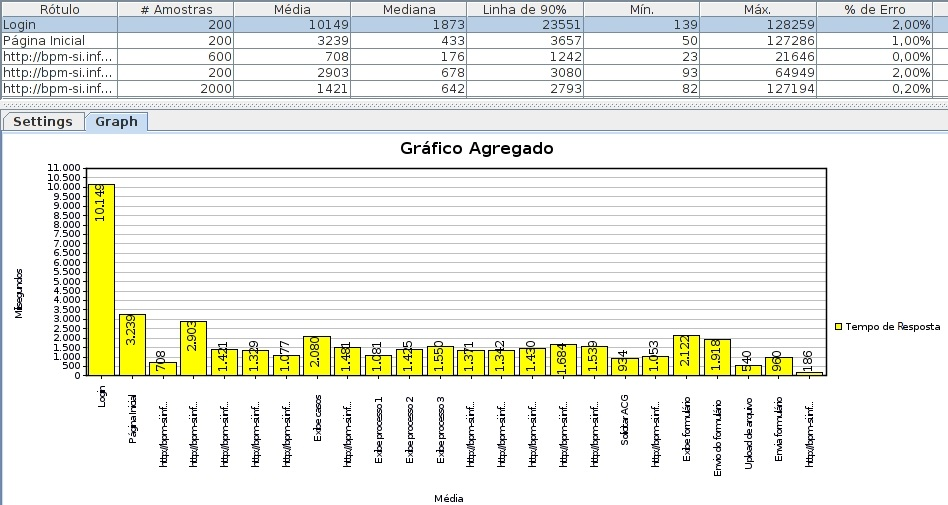
\includegraphics[width=.99\textwidth]{figuras/grafico200.jpg}
%\caption{Resultado dos testes de carga com 200 usuários no JMeter.}
%\label{fig:carga200}
%\end{figure}

Os resultados, em milissegundos, de cada etapa com a variação do número de usuários pode ser visto na Tabela \ref{tab:resultadoCarga}. Os resultados mais alarmantes são os que retratam 200 usuários virtuais, o tempo de resposta médio na requisição que executa o login no sistema foi de 10.149 milissegundos, ou seja, aproximadamente 10 segundos, o que pode ser considerado um tempo de resposta alto. A média de tempo de resposta para todas requisições foi de 3.111 milissegundos (ou seja, 3 segundos), e o desvio padrão foi de 13.088. Além dos altos tempos de resposta, o teste com 200 usuários virtuais apresentou taxas de erro, em algumas requisições, que não foram encontradas com um número menor de usuários. Por exemplo, a requisição que executou login apresentou uma taxa de 2\% de erro e, ao todo, todas requisições obtiveram uma taxa de 7.82\%, o que é preocupante.

De forma geral, portanto, este teste atingiu seus objetivos e serve para explicar um problema que ocorreu no sistema em execução que foi a falha do sistema, onde alguns arquivos foram corrompidos, bem como um tempo de espera muito alto para o aluno acessar o formulário de solicitação. Outro ponto importante é que este teste foi executado apenas no login e na primeira tarefa do processo alvo e, mesmo assim, a tarefa de teste já foi trabalhosa pelo fato de exigir uma análise profunda das requisições para executar os testes com sucesso. A captura destas etapas, utilizando o BlazeMeter\footnote{BlazeMeter. Disponível em: www.blazemeter.com.}, resultou em uma média de 100 requisições, considerando que deseja-se fazer o teste de outra etapa/gargalo que esteja localizada mais ao meio do processo a captura desta pode gerar muitas requisições o que tornaria difícil a análise de todas requisições para substituir as chaves geradas e, assim, tornaria inviável essa abordagem de teste. 

Um fator importante também é que, pelo fato das requisições terem de ser analisadas para ser possível executar o teste e também ser necessário localizar a forma como a ferramenta BPMS implementa a dependência entre as etapas do processo, essa abordagem de teste pode tornar-se muito dependente do BPMS. Esta ideia é fortalecida pela impossibilidade de executar o teste na ferramenta Activiti afinal, dependendo da ferramenta, pode ser muito trabalhoso executar o teste, pode não ser possível executar o teste ou ainda pode ser possível e vantajoso, como ocorreu com o Bonita Open Solution.

\subsection{Teste Funcional}
Para executar os testes funcionais, escolheu-se a ferramenta Selenium\footnote{Selenium. Disponível em: www.seleniumhq.org.}. Esta ferramenta possui basicamente duas partes complementares: Selenium IDE e Selenium WebDriver. A primeira é um plugin para o navegador Firefox, capaz de registrar e reproduzir interações do usuário com o navegador, assim permitindo criar scripts de teste rapidamente, sem escrita de código.


\begin{table}
{\scriptsize
\begin{tabular}{|p{5cm}|p{4cm}|p{4cm}|}
\hline
 & BOS & Activiti \\\hline
Componentes WEB & HTML, CSS, Ajax & HTML, CSS, Ajax \\\hline
Captura da interação do usuário utilizando o Selenium & Total & Parcial (necessitou de inserção manual de alguns campos) \\\hline
Foi possível exportar o código gerado pelo Selenium? & Sim & Sim \\\hline
Reconhecimento de todos os campos capturados SEM alteração de código & Parcial & Parcial \\\hline
Reconhecimento de todos os campos capturados COM alteração de código & Total & Total \\\hline
Foi possível criar o cenário e executar o teste? & Sim & Sim \\\hline
\end{tabular}
}
\caption{Teste funcional}
\label{tab:testeFuncional}
\end{table}

Durante a revisão bibliográfica, encontrou-se um trabalho apresentado no Simpósio Brasileiro de Qualidade de Software de 2013 \cite{sbqs2013} que utilizava o Selenium WebDriver aliado ao Cucumber-JVM\footnote{Cucumber-JVM. Disponível em:www.github.com/cucumber/cucumber-jvm.} para testar uma aplicação web, a partir desse trabalho decidiu-se utilizar a última na execução dos testes funcionais. O Cucumber é uma ferramenta que executa descrições de teste, em texto simples, como testes automatizados.


O processo para a execução do teste funcional é composto por seis etapas: Captura da execução no navegador (Selenium), Exportar código gerado (Selenium), Criar cenário de teste (Cucumber), Criar as definições dos passos do teste (Cucumber), Criar os métodos para cada passo (Java) e Executar o teste (Selenium).

Como o processo testado é o mesmo nos dois BPMS, o cenário de teste também é o mesmo. O cenário nada mais é do que a definição, em ordem de execução, dos passos que são executados na aplicação bem como  os resultados esperados.

Algumas personalizações são necessárias para a execução com sucesso do teste funcional, a maioria delas ocorre nas etapas de exportação/execução do teste. Em ambos os BPMS, ao executar o teste gravado, ocorrem erros pois o Selenium não encontra os campos que ele mesmo capturou. Isto ocorre pois os campos estão localizados dentre de \emph{iframes} que, no momento da captura da interação, não exibem problemas mas na execução acabam por "esconder" os campos, assim é necessário utilizar uma função para "acessar" o \emph{iframe} antes de selecionar o elemento desejado, garantindo que não ocorra erro durante a execução.

%A Figura \ref{fig:codigobos} exibe duas "personalizações" no código gerado pelo Selenium IDE, a primeira (em vermelho) é uma linha de código que faz com que o driver "aguarde"  60 segundos antes de procurar pelo campo a ser selecionado. Isto evita que o driver busque por um campo, antes da página ser carregada, e não o encontre (o que causa erro na execução dos teste). A segunda linha de código, em verde, exibe o código que "acessa" o \emph{iframe}, através da ID, antes de executar a ação e isto também evita que o driver não encontre o elemento no momento do teste.


%\begin{figure}[ht]
%\centering
%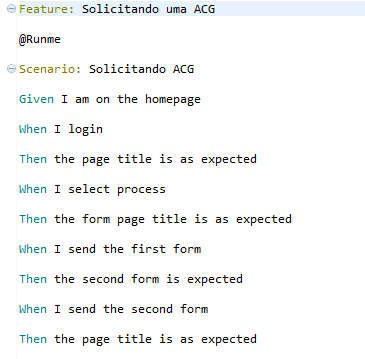
\includegraphics[width=.50\textwidth]{figuras/cenario.png}
%\caption{Cenário de teste}
%\label{fig:cenariobos}
%\end{figure}

Além dos problemas comuns as duas ferramentas citados acima, a ferramenta Activiti demonstrou um outro problema. Diferente da gravação com o BOS, o Selenium IDE não captura toda a interação do usuário com a aplicação, de fato, na etapa de login a IDE captura apenas o acesso a página e o "clique" ao botão de login, ou seja, não captura o preenchimento dos campos "Usuário" e "Senha". Este problema se repete com alguns outros elementos durante a gravação de teste, acredita-se que esse problema ocorra devido a estrutura da página web em questão, estrutura esta que pode conter elementos com os quais o Selenium não trabalhe bem como \emph{divs},\emph{frames} e \emph{scripts}, por exemplo. No entanto, este problema não impossibilita a criação e execução do teste.

Na criação dos métodos correspondentes a cada etapa do processo foi utilizado o código do gerado pelo Selenium IDE mas, como esta não captura todas as interações, a execução do teste falha. Para contornar esse problema, foi necessário estudar a estrutura das páginas que web, localizar os elementos faltantes e então adicionar o código para acessá-los nos respectivos métodos.

\subsubsection{Resultados}

O teste funcional da ferramenta Bonita Open Solution e da ferramenta Activiti mostrou-se mais viável do que o teste de carga, o teste funcional não utiliza chaves identificadoras ou \emph{ids}, como ocorre no teste com o Jmeter, já que uma boa parcela do teste é executada no lado cliente, o que facilita o processo de teste. Pode-se dizer que este teste atingiu todos seus objetivos pois permitiu executar a interação do usuário, bem como criar o código para simular diferentes entradas e testar o a aplicação de diversas formas.

O teste funcional também não é dependente da implementação do BPMS, são necessárias poucas modificações no código gerado e a realização destas é possível apenas inspecionando a estrutura das páginas web.

O Cucumber-JVM torna a implementação dos testes mais rápida e menos trabalhosa, já que a utilização de cenários auxilia na implementação do teste de forma a diminuir a quantidade de código que precisaria ser escrita sem o uso de uma ferramenta como esta.

O teste funcional com o Selenium+Cucumber pode encontrar problemas ao testar várias tarefas ou todos os possíveis fluxos do processo alvo pois, como já foi citado, é necessário fazer algumas modificações no código gerado pelo Selenium e essas modificações, dependendo do volume de tarefas/fluxos, podem ser muito trabalhosas ou até inviabilizar o teste.

%\section{Trabalhos Relacionados}

%artigos sbqs 2014
%artigos sbqs 2013 -

%O teste de software voltado especificamente a aplicações de BPM é um assunto que pode ser considerado ainda em aberto. Atualmente, muitos trabalhos de pesquisa têm focado em etapas de monitoramento e otimização em BPM~\cite{Gambini:2011:AEC:2040283.2040300, Liu:2011:BAM:2040283.2040307, deLeoni:2012:AEL:2413516.2413525, Ramezani:2012:DIM:2413516.2413545}, que são etapas dedicadas a identificar e corrigir problemas. Embora exista alguma relação com testes em BPM, tratam-se geralmente de abordagens mais voltadas a aspectos de gestão, não de software . Por outro lado, um assunto que tem sido bastante abordado é o teste automatizado de aplicações orientadas a serviços Web~\cite{soatest2008}. Embora se trate de um nicho de teste de software, e mesmo que haja uma relação entre BPMS e serviços Web, acredita-se que esta abordagem não abarque toda a problemática do teste de aplicações de BPM. Na aplicação alvo deste trabalho, em particular, a abordagem orientada a serviços Web não poderia ser usada, pois o BPMS empregado baseia-se numa arquitetura que não expõe seus serviços.

%No que diz respeito a relatos de experiência e estudos de caso, costuma haver espaço para isso em conferências internacionais sobre BPM e engenharia de software. Conforme van der Aalst (2013), em uma análise de várias edições da International Conference on Business Process Management, há muitos artigos que descrevem esforços de implementação e estudos de caso. No entanto, vários deles envolvem software que não é disponível ao leitor ou casos que são deliberadamente vagos~\cite{aalst2013survey}. No Brasil, conferências como o Simpósio Brasileiro de Sistemas de Informação e o Simpósio Brasileiro de Engenharia de Software incluem BPM e testes de software entre seus tópicos de interesse mas, até onde foi possível verificar, ainda não foram publicados trabalhos associando esses dois tópicos.

%Embora o termo ``teste'' não seja frequente na literatura sobre BPM, o ciclo de vida de aplicações de BPM inclui as etapas de monitoramento e otimização, que se dedicam a identificar e corrigir problemas~\cite{weske}. Tal visão do ciclo de vida é comumente voltada a aspectos de gestão, não de tecnologia (software). Mesmo assim, acreditamos que o teste de software relacione-se particularmente com essas etapas e, de forma geral, possa contribuir significativamente para o sucesso de aplicações de BPM.

%O artigo 'Um estudo sobre testes de desempenho com aplicação prática utilizando a ferramenta JMeter' (referencia) descreve o resultado de um estudo sobre testes de desempenho aplicado teste de desempenho aplicado em uma arquitetura e-commerce hipotética utilizando o JMeter. Diferentemente do presente trabalho, este artigo não possui usuários e um sistema real para ser analisado, sendo seu o objetivo analisar os dados para o desenvolvimento de um aplicativo, não para a melhoria do sistema.

%selenium e JMeter
%No trabalho “A Test Automation Framework Based on Web” \cite{wang2012test} é relatada a criação de um framework para teste automatizado de aplicações web, utilizando as ferramentas Selenium e JMeter. Os resultados do trabalho demonstram que as ferramentas ajudam, bem como o framework, ajudam a melhorar a qualidade do software e a aumentar a eficiência do desenvolvimento.

%testes com Selenium;
%O artigo “Automating functional tests using Selenium”\cite{holmes2006automating} é um relato de experiência utilizando o Selenium para testes automatizados e descreve as dificuldades e aprendizados com esta ferramenta, como tempo para escrever os scripts de teste bem como integração. Entretanto, os testes são baseados em aplicações Web simples e não em BPM. De fato não foram encontrados artigos que unissem BPM e a ferramenta Selenium para testar processos.

%trabalhos mais teoricos sobre teste de BPM (possivelmente citar na Seção 2)
%No white-paper “Performance Testing of Business Process Management (BPM) aplications using JMeter” \cite{} é um artigo teórico que defende a importância do teste de performance nas aplicações baseadas em BPM, para evitar a falha dos processos no ambiente de produção, bem como defende o uso do JMeter para implementar os testes levantando várias justificativas, dentre elas o fato de ser uma ferramenta gratuita que tem tantas funcionalidades quanto ferramentas pagas. Diferente do nosso trabalho, este não possui um ambiente em produção ou um processo real, com problemas reais, para efetuar o teste com o JMeter. O trabalho apenas trata da importância dos testes e sobre a potencialidade do JMeter.

\section{Conclusão}
O maior objetivo deste trabalho foi explorar soluções para teste automatizado de aplicações em BPM. Pode se dizer que esse objetivo foi atingido pois, durante a execução do trabalho, foi possível obter várias conclusões sobre o teste automatizado deste tipo de software.

%Uma das abordagens adotadas foi de que, por aplicações BPM serem aplicações WEB, poderiam ser tratadas e testadas como um software em geral, utilizando ferramentas consagradas para tal. De fato, esta abordagem mostrou algumas desvantagens e dificuldades relacionadas a particularidades das aplicações BPM.

Sobre o ponto de vista do teste de carga, o teste mostrou-se útil para explicar falhas ocorridas no sistema que foi implementado. Também mostrou-se um teste trabalhoso, ou até inviável, dependendo do número de tarefas no processo e do BPMS. A experiência com duas ferramentas fortaleceu essa conclusão pois ocorreram duas situações distintas, com o Bonita Open Solution o teste mostrou-se válido porém, com o BPMS Activiti o teste foi impossível de ser executado. O BPMS deve ser avaliado antes da execução do teste para verificar se este é vantajoso ou não.

No teste funcional obteve-se maior sucesso na execução dos testes pois a dependência das ferramentas BPMS na criação dos testes é menor. A tarefa de teste pode vir a ser trabalhosa, principalmente quando deseja-se testar todas tarefas e fluxos possíveis que um processo de negócio pode ter.
%\begin{figure}[ht]
%\centering
%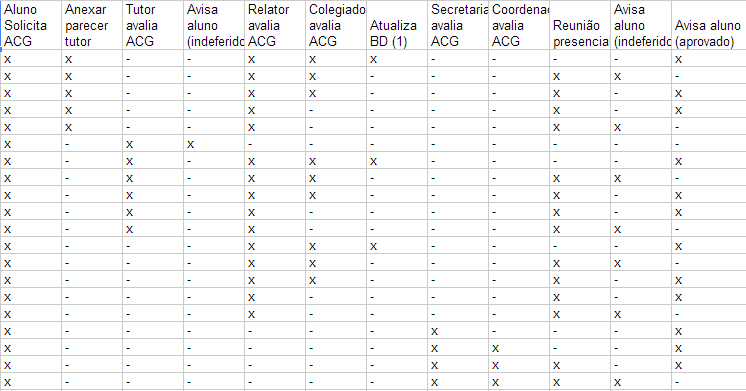
\includegraphics[width=.99\textwidth]{figuras/tabelaCaminhos.png}
%\caption{Possíveis caminhos}
%\label{fig:tabelaCaminhos}
%\end{figure}
%Nas ferramentas abordadas no neste trabalho ou nas ferramentas estudadas e tabeladas, não foi encontrado nenhum tipo de suporte a teste automatizado dos processos, uma particularidade dos processos é que estes podem possuir diversos caminhos e estes caminhos precisam ser testados. Na Tabela \ref{tab:tabelaCaminhos} foram exibidos cujos testes foram executados manualmente e, com base no estudo executado neste trabalho e nas ferramentas estudadas, pode-se afirmar que atualmente é muito difícil encontrar um BPMS com suporte a este tipo de teste.

Com o aprofundamento nas ferramentas abordadas nesse trabalho, pode se afirmar que o campo de teste automatizado em ferramentas BPMS ainda é pouco explorado mas, como foi visto na aplicação citada, aplicações BPM estão suscetíveis a erros tanto quanto outras aplicações e poderiam se beneficiar com o avanço desta área.

%Como trabalhos futuros, pode-se destacar a continuação exploração de ferramentas de geração de casos de teste, na hipótese de que possam ajudar a alinhar os testes com as saídas e entradas do processo. Outra via que merece ser explorada são os testes de regressão, para auxiliar a encontrar possíveis problemas após alterações no processo, que podem ser frequentes dependendo do caso.


\bibliographystyle{sbc}
\bibliography{sbc-template}


\end{document}





